\documentclass[10pt]{article}
\usepackage[utf8]{inputenc}
\usepackage[T1]{fontenc}
\usepackage{amsmath}
\usepackage{amsfonts}
\usepackage{amssymb}
\usepackage[version=4]{mhchem}
\usepackage{stmaryrd}
\usepackage{bbold}
\usepackage{graphicx}
\usepackage[export]{adjustbox}
\graphicspath{ {./images/} }

\begin{document}
(8)

Nate that, because of symmetry, the s-point carrelation for $s$ any odd integer is fero (the Gaussion remains unchanged if $\vec{x} \rightarrow-\vec{x})$.

What happens when we want to calculate $\left\langle x_{i} x_{j} \cdots x_{e}\right\rangle$ ? Should we always do all the derivatives as in ep. (12)? No!\\
of the vars are Goussion we can use

Wick's theorem: Any correlation between an even number of Gaussion 2. V. can be written down as a sum of products of 2- point conelation functions $\left(A^{-1}\right)$.\\
For instance

$$
\begin{aligned}
\left\langle x_{a} x_{b} x_{c} x_{d}\right\rangle= & \left\langle x_{a} x_{b}\right\rangle\left\langle x_{c} x_{d}\right\rangle+\left\langle x_{a} x_{c}\right\rangle\left\langle x_{b} x_{d}\right\rangle+\left\langle x_{a} x_{d}\right\rangle\left\langle x_{b} x_{c}\right\rangle \\
& \left.\left(A^{-1}\right)_{a b} \quad \hat{~}_{A^{-1}}\right)_{c d} \quad \cdots \quad \text { (indexes may be equal) }
\end{aligned}
$$

Exercize: from the previous cose, show that (no calculations!)

$$
\begin{aligned}
& \left\langle x_{1}^{2} x_{2}^{2}\right\rangle=\frac{3}{8} \cdot \frac{3}{8}+\frac{1}{8} \cdot \frac{1}{8}+\frac{1}{8} \cdot \frac{1}{8}=\frac{11}{64} \\
& \left\langle x_{1}^{4}\right\rangle=3\left(\frac{3}{8}\right)^{2}=\left\langle x_{2}^{4}\right\rangle,\left\langle x, x_{2}^{2}\right\rangle=0
\end{aligned}
$$

In general:\\
(14) $\langle\underbrace{x_{i} x_{j} \ldots x_{n} x_{m}}_{s \text { vors }}\rangle=\sum_{p}\left(A^{-1}\right)_{i_{p} j_{p}} \cdots\left(A^{-1}\right)_{n_{p} m_{p}}$

Where the sum uns over all pairings of $s$ indexes, i.e. over all ways of grouping $s$ (even) indexes $i, j \cdots, n, m$ into poins (counting the poin even when indexes are equal; order in the poirs is not important). Of there are $s$ vers then the passible painings are $(s-1)!!=(s-1)(s-3) \ldots 3.1$.

Further important results obtained with choracteristic functions\\
(1) If you are given two indipendent and identically distributed (iit) roudom variables, how do you calculate the polf of thein sum? What is its c.f.?\\
We assume they are real with pof $q(x)$ :\\
2.v. drawn from

$$
x=x_{1}+x_{2} \quad x_{1}, x_{2} \stackrel{\downarrow}{\sim} g(x)
$$

When we dow $x_{1}$ and $x_{2}$ from $q(x)$, many different outcomes con give you the same sum $x$, these have to be added up with the consesponding probability, hence\\
(15) $p(x)=\int \delta(x-\left(x_{1}+x_{2}\right) \underbrace{q\left(x_{1}\right) q\left(x_{2}\right)} d x_{1} d x_{2} \equiv\left\langle\delta\left(x-x_{1}-x_{2}\right)\right\rangle$

$$
=\int q(x-y) q(y) \text { because they are iid }
$$

What is the c.f. of $p(x)$ if the c.f. of $q(x)$ is $\varphi_{1}(k)$ ?\\
(16)

$$
\begin{aligned}
\varphi(k) & \equiv\left\langle e^{i k x}\right\rangle=\int p(x) e^{i k x} d x=\int d x e^{i k x} \delta\left(x-\left(x_{1}+x_{2}\right)\right) q\left(x_{1}\right) q\left(x_{2}\right) d x_{1} d x_{2} \\
& =\int e^{i k\left(x_{1}+x_{2}\right)} q\left(x_{1}\right) q\left(x_{2}\right) d x_{1} d x_{2}=\left[\varphi_{1}(k)\right]^{2}
\end{aligned}
$$

What happens if the $2 . v$. are independ. but not identically distributed?\\
(10) The (weak) law of large numbers (converg. in distrib.)\\
(2) If we are now given $n$ iiid $2 . v$. whose polf is $q(x)$ with c.f. $\varphi_{1}(x)$, what happens to $x=\frac{1}{n} \sum_{i} x_{i} x_{i}$ as $n \rightarrow \infty$ ?\\
Let's assume that the mean of $x_{i}$ is $\mu \quad\left(\mu=\int x q(x) d x\right)$.\\
All calculations are simples if we use the $c-f$. of $x$. (See Grimmett, p. 193)\\
$\varphi(k) \equiv\left\langle e^{i k x}\right\rangle=\left\langle e^{i k \frac{1}{n} \sum_{i} x_{i}}\right\rangle=\int e^{i \frac{k}{n} \sum_{i} x_{i}} q\left(x_{1}\right) \ldots q\left(x_{n}\right) d x_{1} \ldots d x_{n}$\\
(17) $=(\underbrace{\int e^{i \frac{k}{n} x_{1}} q(x) d x}_{\varphi_{1}\left(\frac{k}{n}\right)}) \cdots\left(\int e^{i \frac{k}{n} x_{n}} q\left(x_{n}\right) d x_{n}\right)=\left[\varphi_{1}\left(\frac{k}{n}\right)\right]^{n}$

Also, Taylor

$$
\varphi_{1}\left(\frac{k}{n}\right) \equiv \int e^{i \frac{k}{n} x} q(x) d x \stackrel{\downarrow}{=} 1+\frac{i k}{n}\langle x\rangle+\sigma\left(\frac{1}{n}\right) \text { as } n \rightarrow \infty
$$

From (17)

$$
\begin{aligned}
& \left(1+\frac{i k}{n} \mu+\theta\left(\frac{1}{n}\right)\right)^{n} \\
& \text { by proved that } \varphi_{n}(k) \rightarrow e^{i \mu k},-n \rightarrow \infty
\end{aligned} e^{i \mu k}=\underbrace{\int(x-\mu) e^{i k x} d x}_{\rho(x)}
$$

Here we have only proved that\\
We have a much stronger result:\\
(18) $\frac{1}{n} \sum_{i}^{n} x_{i} \rightarrow \mu$ The strong law of loye numbers stotes Let $x_{1} \ldots x_{m}$ be a sequence of i.i.d. z.v. each with finite mean $\mu$. Then the finite (empinical) overoge approaches $\mu$ as $n \rightarrow \infty$. (Grimmett, p. ${ }^{329}$ )\\
This law tells us that, for large $n$, the sum $\sum_{i} x_{i}$ is approximately $x \mu$. Of cousse there will be fluctuations around $n \mu$. A natural question is then what can we say about $\sum_{i}^{n} x_{i}-\mu n$ ?\\
There is an extraorolinary answer to this question, which is valid whenever $x_{i}$ have finite veriance:\\
a) $\sum_{i}^{m} x_{i}-\mu n$ is about as big as $\sqrt{n}$\\
b) The distribution of $\frac{\sum_{i}^{n} x_{i}-\mu n}{\sqrt{n}}$ approaches a Gaussian polf as $n \rightarrow \infty$ IRRESPECTIVE of the pof of $x_{i}$.

Claims a) and b) ore the core meaning of the

\section*{Central Limit Theorem}
Let $x_{1} \ldots x_{n}$ be a sepvence of i.i.d. n.v. with finite mean $\mu$ and finite (non-zero) variance $\sigma^{2}$. Then the p.d.f. of\\
(19) $\quad Y_{n}=\frac{\sum_{i}^{m} x_{i}-\mu n}{\sqrt{n} \sigma} \xrightarrow[n \rightarrow \infty]{ } N(0,1)$ (Gaussion polf with mean 0)

Obs: $\left\langle Y_{n}\right\rangle=\frac{1}{\sqrt{n} \sigma}\left(\sum_{i}^{n}\left\langle x_{i}\right\rangle-\mu_{n}\right)=0$

$$
\operatorname{Var}\left(Y_{n}\right)=\frac{1}{n \sigma^{2}} \operatorname{Var}\left(\sum_{i}^{m} x_{i}-\mu m\right)=\frac{1}{m \sigma^{2}} \operatorname{Var}\left(\sum_{i}^{m} x_{i}\right)=\frac{\tilde{\sum}_{i} \operatorname{Var}\left(x_{i}\right)}{n \sigma^{2}}=\frac{n \sigma^{2}}{n \sigma^{2}}=1
$$

(please, go throughly through all the steps and uvise the properties of var (…)).\\
This means that $Y_{n}$ has a center (0) and a "width" that does not chage as $n$ varies.\\
We use the properties of c.f. to prove this theoreen. Let's assume that each z.v. has a p.d.f $q(x)$ with c.f. $\varphi_{1}(k)$. Then


\begin{align*}
\varphi(k) & =\left\langle e^{i k V_{n}}\right\rangle=\int e^{i k \frac{\sum_{i} x_{1}-\mu n}{\sqrt{n} \sigma}} q(x,) \cdots q\left(x_{n}\right) d x, \cdots d x_{n}= \\
& =e^{-\frac{i k \mu \sqrt{n}}{\sigma}}(\underbrace{\int e^{i \frac{k}{\sqrt{n} \sigma} x} q(x) d x}_{\varphi_{i}\left(\frac{k}{\sqrt{n} \sigma}\right)})^{n} \tag{20}
\end{align*}


As we have seen in the previous theorem, as $n \rightarrow \infty$ Taylar

$$
\begin{aligned}
\varphi_{1}\left(\frac{k}{\sqrt{n} \sigma}\right) & \stackrel{\downarrow}{=} 1+\frac{i k}{\sqrt{n} \sigma}<x>-\frac{k^{2}}{2 n \sigma^{2}}<x^{2}>+O\left(x^{-3 h}\right) \\
& =e^{\frac{i k}{\sqrt{n} \sigma} \mu-\frac{k^{2}}{2 n}} \quad\left(<- \text { show why only }-\frac{k^{2}}{2 n} \text { zemoins. }\right)
\end{aligned}
$$

From of. (20)

$$
\varphi(k)=e^{-\frac{i k \mu}{\sigma} \sqrt{n}} \quad e^{\frac{i k \mu}{\sigma} \sqrt{n}-\frac{k^{2}}{2}}=e^{-\frac{k^{2}}{2}}
$$

As we have shown in ep. (6), this is the e.f. of $p(x)=\frac{1}{\sqrt{2 \pi}} e^{-\frac{x^{2}}{2}} \equiv N(0,1)$ Show 1) $\sum_{i}^{n} x_{i} \sim N\left(n \mu, n \sigma^{2}\right) ;$ 2) $\frac{1}{n} \sum_{i} x_{i} \sim N\left(\mu, \frac{\sigma^{2}}{n}\right)$.

\section*{The Laplace Method}
In many situations, one weeds to evaluate complicated integuals of the frum


\begin{equation*}
I(\lambda)=\int_{x_{1}}^{x_{2}} d x g(x) e^{\lambda f(x)} \quad \lambda \in \mathbb{R} \tag{21}
\end{equation*}


Although $I(\lambda)$ comnot be coluclated for an arbitrary $\lambda$, it happens that it con be well approximated as $\lambda \rightarrow \infty$.\\
the cree idea of Loplace's method is that the major contribution to the integral in (21) as $\lambda \rightarrow \infty$ comes from the reighbousheed of the point in $\left[x_{1}, x_{2}\right]$ where $f(x)$ attrins its moximum value.

There are esentially 3 coses:\\
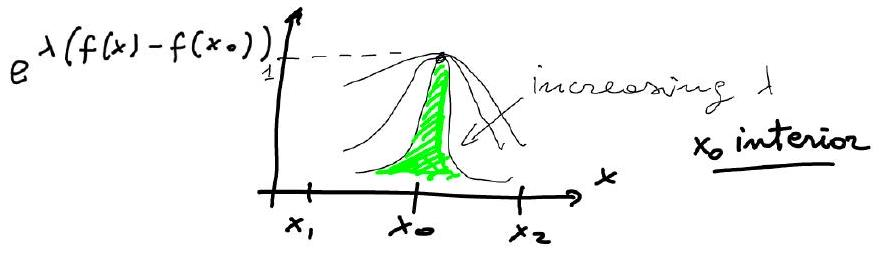
\includegraphics[max width=\textwidth, center]{2025_10_17_86b952e516931f75c0b7g-05}

\begin{enumerate}
  \item $x_{1}<x_{0}<x_{2}$, $x_{0}$ interior, and $f^{\prime}\left(x_{0}\right)=0$. We also assume $f^{\prime \prime}\left(x_{0}\right)<0$ (why?) (actually if $f^{\prime}\left(x_{0}\right)=f^{\prime \prime}\left(x_{0}\right)=f^{\prime \prime \prime}\left(x_{0}\right)=0$ but $f^{(11)}\left(x_{0}\right)<0$ is not more diff) and $g\left(x_{0}\right) \neq 0$ and finite. $f$ is continuously differ. in $\left[x_{1}, x_{2}\right]$.\\
As we expect that the dominani pert comes from the neighbounhood of $x_{0}$ and $f(x)=f\left(x_{0}\right)+\frac{\left(x-x_{0}\right)^{2}}{2} f^{\prime \prime}\left(x_{0}\right)+o\left(1-\left.x_{0}\right|^{2}\right)$ as $x \rightarrow x_{0}$, we approximate\\
$I(\lambda) \simeq \int_{x_{1}}^{x_{2}} g(x) e^{\lambda\left(f\left(x_{0}\right)+\frac{\left(x-x_{0}\right)^{2}}{2} f^{\prime \prime}\left(x_{0}\right)\right)} d x=g\left(x_{0}\right) e^{\lambda f\left(x_{0}\right)} \int_{x_{1}}^{x_{2}} e^{-\lambda \frac{\left(x-x_{0}\right)^{2}}{2}\left(f^{\prime \prime}\left(x_{0}\right)\right)} d x$\\
We chage ver: $\quad s=\left(x-x_{0}\right) \sqrt{\frac{\left|f^{\prime \prime}\left(x_{0}\right)\right| \lambda}{e}}$ hence
\end{enumerate}

$$
\left(x_{2}-x_{0}\right) \sqrt{\frac{f^{4}\left(x_{a}-1\right)}{2}}
$$

$I(\lambda) \simeq g\left(x_{0}\right) e^{\lambda f\left(x_{0}\right)} \sqrt{\frac{2}{\lambda\left|f^{\prime \prime}\left(x_{0}\right)\right|}} \int e^{-s^{2}} d s$

$$
\left(x_{1}-x_{0}\right) \sqrt{f^{\prime \prime}\left(x_{0}\right) \mu}
$$

$\xrightarrow[\lambda \rightarrow \infty]{ } \int_{-\infty}^{+\infty} e^{-s^{2}} d s=\sqrt{\pi}$ with exp. swoll enors.

$$
I(t) \simeq g\left(x_{0}\right) e^{\lambda f\left(x_{0}\right)} \sqrt{\frac{2 \pi}{\lambda\left|f^{\prime \prime}\left(x_{0}\right)\right|}}
$$

as $\lambda \rightarrow+\infty$ (leading order)

Exercige: Con you show that a better approximation is given by

$$
I(\lambda) \simeq e^{\lambda f\left(x_{0}\right)} \sqrt{\frac{2 \pi}{\lambda\left|f^{\prime \prime}\left(x_{0}\right)\right|}}\left(g\left(x_{0}\right)+\frac{c}{\lambda}\right) \quad \text { os } \quad \lambda \rightarrow+\infty
$$

Where $c$ is a construct that depends on derivatives of $f(x)$ up to $4^{\text {th }}$ onder (at $x=x_{0}$ ) and on $g\left(x_{0}\right)$ and $g^{\prime}\left(x_{0}\right)$ ?\\
2) $x_{0}=x_{1}$ or $x_{0}=x_{2}$ ( $x_{0}$ is an endpoint) and $f^{\prime}\left(x_{0}\right)=0, f^{\prime \prime}\left(x_{0}\right)<0$. Then\\
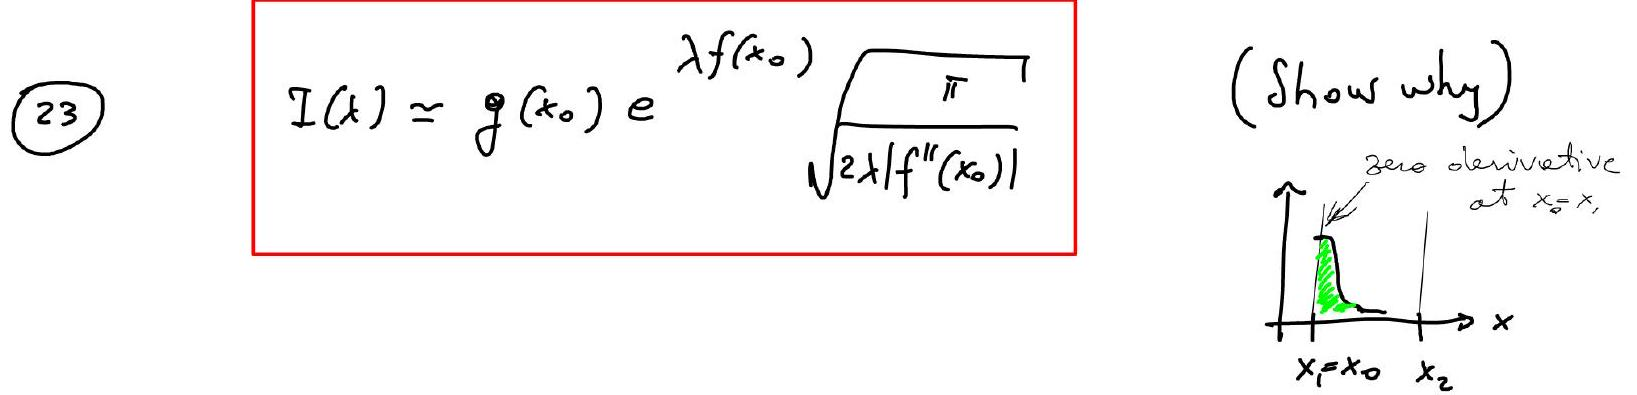
\includegraphics[max width=\textwidth, center]{2025_10_17_86b952e516931f75c0b7g-06}

\section*{Example:}
\begin{center}
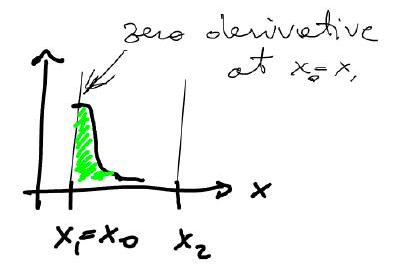
\includegraphics[max width=\textwidth]{2025_10_17_86b952e516931f75c0b7g-06(1)}
\end{center}

The madified Bessel function of the second kind is a special function that occurs in many applications. There exists an integral represent.:

$$
K_{\nu}(x)=\int_{0}^{\infty} e^{-x \cosh t} \cosh (\nu t) d t
$$

We wish to estimate $k_{\nu}(x)$ as $x \rightarrow+\infty$ for fixed $\nu$.\\
Since $\cosh ^{\prime}(t)=\sinh (t)>0$ for $t>0$, the max of $e^{-x \cosh t}$ as a function of $t$ (for fixed $x>0$ ) occurs at $t=0$ (the left edge). So we con apply (23)

$$
\begin{aligned}
& \cosh t \simeq 1+\frac{t^{2}}{2}+\text { h.o.t. } \\
& k_{2}(x) \simeq e^{-x} \sqrt{\frac{\pi}{2 x}} \quad \text { as } x \rightarrow \infty \\
& \text { at leoding onder }
\end{aligned}
$$

notice that it does not depend on $\nu$ !\\
Show that

$$
k_{\nu}(x)=\sqrt{\frac{\pi}{2 x}} e^{-x}\left(1+\frac{c(\nu)}{x}+\cdots\right)
$$

and colculate $c(\nu)=\frac{4 \nu^{2}-1}{8}$.\\
(14)\\
( $x_{0}$ an endpoint)\\
3) $x_{0}=x_{1}$ or $x_{0}=x_{2}$ but $f^{\prime}\left(x_{0}\right) \neq 0$.\\
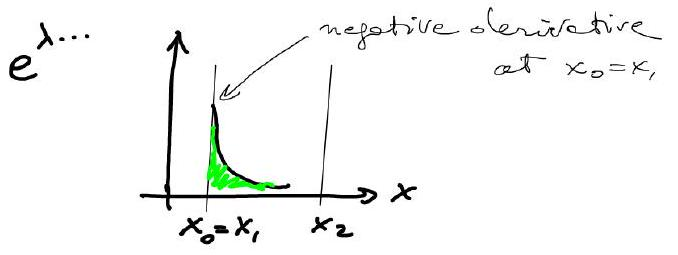
\includegraphics[max width=\textwidth, center]{2025_10_17_86b952e516931f75c0b7g-07}\\
Without lass of generality, let's say that $x_{0}=x_{1}$ and $f^{\prime}\left(x_{0}\right)<0$ (why?). Then $f(x)=f\left(x_{0}\right)+\left(x-x_{0}\right) f^{\prime}\left(x_{0}\right)+\cdots$ and\\
$I(\lambda) \simeq \int_{x_{1}=x_{0}}^{x_{2}} g(x) e^{\lambda\left[f\left(x_{0}\right)+\left(x-x_{0}\right) f^{\prime}\left(x_{0}\right)+\cdots\right]} d x=g\left(x_{0}\right) e^{\lambda f\left(x_{0}\right)} \int_{x_{1}=x_{0}}^{x_{2}} e^{\lambda\left(x-x_{0}\right) f^{\prime}\left(x_{0}\right)} d x S=x-x_{0}$\\
$=g\left(x_{0}\right) e^{\lambda f\left(x_{0}\right)} \int_{0}^{x_{2}-x_{1}} e^{\lambda s f^{\prime}\left(x_{0}\right)} d s=g\left(\frac{x_{0}}{\lambda f^{\prime}\left(x_{0}\right)} e^{\lambda f\left(x_{0}\right)}\left[e^{\lambda s f^{\prime}\left(x_{0}\right)}\right]_{0}^{x_{2}-x_{1}}=\right. =\frac{g\left(x_{0}\right) e^{\lambda f\left(x_{0}\right)}}{\lambda f^{\prime}\left(x_{0}\right)}\left(e^{\lambda\left(x_{2}-x_{1}\right) f^{\prime}\left(x_{0}\right)}-1\right)$\\
As $\lambda \rightarrow+\infty$ use get (with exp. swall tesms)\\
(2n) $I(\lambda) \simeq g\left(x_{1}\right) \frac{e^{\lambda f\left(x_{1}\right)}}{\lambda\left|f^{\prime}\left(x_{1}\right)\right|} \quad$ os $\lambda \longrightarrow \infty$

Multiple maxima in $\left[x_{1}, x_{2}\right]$ with equal value can be dealt with similarly.

Example:\\
Obtain the leading order approx. of

$$
I(\lambda)=\int_{0}^{1} x^{m} e^{\lambda\left(3 x^{2}+2 x^{3}\right)} d x \quad \text { as } \lambda \rightarrow+\infty
$$

fixed $m$\\
the max is at $x=1$ with $f(1)=5, f^{\prime}(1)=12, g(1)=1$. We con apply ep. (24)

$$
I(\lambda) \simeq \frac{e^{5 \lambda}}{12 \lambda} \quad(\text { no dependence on } m)
$$

\section*{Stinling's formula}
We would like to understand how fast N! gaes to infinity as $N$ grows. We will do it by applying Laplace's method to the gemme function, which is defined as


\begin{equation*}
\Gamma(\lambda)=\int_{0}^{\infty} x^{\lambda-1} e^{-x} d x \quad \lambda>0 \tag{25}
\end{equation*}


Exercige: show that $\Gamma(\lambda+1)=\lambda \Gamma(\lambda)$, hence $\lambda!=\Gamma(\lambda+1)$ which generalifed the factorial to real (and complex) numbers.

Let's consider $\Gamma(\lambda+1)=\int_{0}^{\infty} x^{\lambda} e^{-x} d x$. If we write it as $\int_{0}^{\infty} e^{-x} e^{\lambda \ln x} d x$ we camat apply Laplace's methad (why?).\\
Instead it is more beneficial if we consider the moximum of the function $f(x)=-x+\lambda \ln x$ and $g(x)=1$. The mox occurs at $x=\lambda$, which suggests a chaye of ver: $x=\lambda t$ (so that the max does no longer depends on $\lambda$ and is fixed):

$$
\begin{aligned}
\Gamma(\lambda+1) & =\int_{0}^{\infty} x^{\lambda} e^{-x} d x \prod_{x=\lambda t} \lambda^{\lambda+1} \int_{0}^{\infty} t^{\lambda} e^{-\lambda t} d t \\
t^{\lambda} e^{-\lambda t} & =e^{\lambda(\ln t-t)}, \quad h(t)=\ln t-t, h^{\prime}(1)=0, h^{\prime \prime}(1)=-1
\end{aligned}
$$

so we con now apply es. (22) with $g(t)=1$ and $t_{0}=1$.\\
(26) $\Gamma(\lambda+1)=\lambda!\simeq \lambda^{\lambda+1} e^{-\lambda} \sqrt{\frac{2 \pi}{\lambda}}$ as $\lambda \rightarrow+\infty$\\
which is the Stilling's famula. We can improve it with a factor $\left(1+\frac{1}{12 \lambda}\right)$\\
Exercize: show that at leading onder

$$
\int_{0}^{\infty} e^{-\lambda t} e^{-\frac{1}{t}} d t \simeq \frac{\sqrt{\pi} e^{-2 \sqrt{\lambda}}}{\lambda^{3 / 4}} \quad \text { as } \quad \lambda \rightarrow+\infty .
$$

$L_{p}$-now in real analysis\\
The quantity

$$
\|g\|_{p}:=\left(\int_{a}^{b}|g(t)|^{p} d t\right)^{1 / p}
$$

is known as Lp-norm in real analyris. The integrand exists in Lebesgue sense. We want to study the behavior of $\|g\|_{p}$ as $p \rightarrow \infty$ When $g$ has a unique assal. max. at the interior point $t_{0}$ and $g \in C^{4}(a, b)$. We finst study

$$
I(p)=\int_{a}^{b}|g(t)|^{p} d t \quad\|g\|_{p}=I(p)^{1 / p}
$$

Then

$$
I(p)=\int_{a}^{b} e^{p \ln |g(t)|} d t
$$

In the application of the Laplace method we assumed that $f$ is contin. diff. If $g$ vanishes somewhere in $[a, b]$ then $\ln |g| \rightarrow-\infty$. However every neighborked of points where $g=0$ will yield a negligible contribution to I for lage $p$. Thus such discontinuities can be neglected. We can opply ep. (22) with $g(t)=1$

$$
\begin{aligned}
I(p) & =e^{p \ln \left|g\left(t_{0}\right)\right|} \sqrt{\frac{2 \pi\left|g\left(t_{0}\right)\right|}{p\left|g^{\prime \prime}\left(t_{0}\right)\right|}}\left(1+O\left(\frac{1}{p}\right)\right) \\
& =\left|g\left(t_{0}\right)\right|^{p} \sqrt{\frac{2 \pi\left|g\left(t_{0}\right)\right|}{p\left|g^{\prime \prime}\left(t_{0}\right)\right|}}\left(1+O\left(\frac{1}{p}\right)\right) \quad \text { as } p \rightarrow \infty
\end{aligned}
$$

Since $\quad a^{1 / p} p^{-\frac{1}{2 p}}=e^{\frac{\ln a}{p}} e^{-\frac{\ln p}{2 p}} \simeq\left(1+\frac{\ln a}{p}+\cdots\right)\left(1-\frac{\ln p}{2 p}+\cdots\right) \simeq 1-\frac{\ln p}{2 p}+\operatorname{lot} I(p)^{1 / p}=\left|g\left(t_{0}\right)\right|\left(\frac{2 \pi|g|}{p\left|g^{\prime \prime}\right|}\right)^{\frac{1}{2 p}}+\operatorname{hot}=\left|g\left(t_{0}\right)\right|\left(1-\frac{\ln p}{2 p}+O\left(\frac{1}{p}\right)\right)$ os $p \rightarrow \infty$\\
hence

$$
\|g\|_{p}=\max _{t \in[a, b]}|g(t)|\left\{1-\frac{\ln p}{2 p}+O\left(\frac{1}{p}\right)\right\} \quad \text { as } p \rightarrow \infty .
$$

Consider the integral

$$
I(\lambda)=\int_{0}^{\frac{3 \pi}{2}} e^{-\lambda \sin t} f(t) d t
$$

Where $f(t)$ is contin. diff. in $\left[0, \frac{3 \pi}{2}\right]$. We have to casider the contributions from the endpoint minima $t=0, \frac{3 \pi}{2}$. Let's write

$$
I(\lambda)=\underbrace{\int_{0}^{\frac{\pi}{2}} e^{-\lambda \sin t} f(t) d t}_{I_{1}}+e^{\lambda} \underbrace{\int_{\pi / 2}^{3 \pi / 2} e^{-\lambda \sin t-\lambda} f(t)}_{I_{2}} d t
$$

Eq. (24) $I_{1}(\lambda)=f(0) \frac{e^{\lambda \cdot 0}}{\lambda|\cos (0)|} \cong \frac{f(0)}{\lambda}$ as $\lambda \rightarrow \infty$

$$
I_{2}(\lambda)=f(3 \pi / 2) e^{\lambda \cdot 0} \sqrt{\frac{\pi}{2 \lambda\left|\sin \left(\frac{3 \pi}{2}\right)\right|}} \cong f\left(\frac{3 \pi}{2}\right) \sqrt{\frac{\pi}{2 \lambda}} \quad \text { as } \lambda \rightarrow \infty
$$

Hence the leading contribution comes from $I_{2}$ and

$$
I(\lambda) \simeq f\left(\frac{3 \pi}{2}\right) e^{\lambda} \sqrt{\frac{\pi}{2 \lambda}}+\text { h.o.t. as } \lambda \rightarrow \infty
$$

The min at $t=0$ is sublasting and should be taken into account only at higher onder.

\section*{Example :}
Let's counder the clan of integrals

$$
I_{m}(x)=\int_{0}^{\infty} t^{m} e^{-\frac{t^{2}}{2}-\frac{x}{t}} d t \quad x>0
$$

ve want to evaluate $I_{m}(x)$ as $x \rightarrow+\infty$ with fixed $m$.\\
The function $\frac{t^{2}}{2}+\frac{x}{t}$ has a movable mini at $\frac{d}{d t}\left(t^{2}+\frac{x}{t}\right)=0, E=x^{1 / 3}$ So we change var. for fixing the min.

$$
t=x^{1 / 3} \tau
$$

So $I_{m}(x)$ can be recost in the frum

$$
I_{m}(x)=x^{\frac{(m+1)}{3}} \int_{0}^{\infty} \tau^{m} e^{-x^{2 / 3}\left(\frac{\tau^{2}}{2}+\frac{1}{\tau}\right)} d \tau
$$

The mine of $\frac{\tau^{2}}{2}+\frac{1}{\tau}$ occurs at $\tau=1$ (interver), so we con opply eq. (22)

$$
\begin{aligned}
I_{m}(x) & \simeq x^{\frac{m+1}{3}} e^{-\frac{3}{2} x^{2 / 3}} \sqrt{\frac{2 \pi}{x^{2 / 3} \cdot 3}} \quad \text { as } x \rightarrow+\infty \\
& =x^{m / 3} e^{-\frac{3}{2} x^{2 / 3}} \sqrt{\frac{2 \pi}{3}}
\end{aligned}
$$

at leashing order in $x$ with fixed $m$.

Show also that as $\lambda \rightarrow+\infty$

$$
\begin{aligned}
& \int_{-2}^{0} e^{t} e^{\lambda\left(3 t^{2}+2 t^{3}\right)} d t \simeq e^{\lambda-1} \sqrt{\frac{\pi}{3 \lambda}} \\
& \int_{0}^{1} e^{t} e^{\lambda\left(3 t^{2}+2 t^{3}\right)} d t \simeq \frac{e^{5 \lambda+1}}{12 \lambda} \\
& \int_{0}^{1} \sqrt{1+t} e^{\lambda\left(2 t-t^{2}\right)} d t \simeq e^{\lambda} \sqrt{\frac{\pi}{2 \lambda}}
\end{aligned}
$$


\end{document}